\subsection{Mesher}
\label{sec:modules_mesher}
Il \emph{mesher} è il componente che, a partire dai dati forniti dal processo di fresatura, crea la mesh 3D dell'oggetto lavorato. Le interfacce di comunicazione con il \emph{miller} e il modulo che visualizzerà la scena sono state definite in maniera precisa: ciò permette la scrittura di \emph{mesher} differenti che ---scelti all'avvio del software--- permettono di rappresentare i voxel non cancellati, piuttosto che una ricostruzione del taglio eseguito. In quest'ultimo caso il mesher si avvale dell'algoritmo Marching Cubes, descritto in sezione \ref{mcalgo}.

La mesh è costruita con gli strumenti messi a disposizione dalla libreria \osg: si tratterà quindi di un albero sui cui rami e sulle cui foglie sono contenute tutte le informazioni necessarie alla rappresentazione grafica dell'oggetto lavorato. Per la struttura dell'albero si è scelto nuovamente un octree non bilanciato in cui le foglie, stavolta, contengono una molteplicità di voxel: quando il numero di oggetti contenuti in una foglia raggiunge un valore di soglia, viene aggiunto un nuovo livello all'albero, ripartendo tra i nuovi figli così creati il volume di competenza ed i voxel precedentemente contenuti. Questa scelta permette di ottimizzare l'uso delle risorse grafiche in quanto limita l'estensione dell'albero della scena e diminuisce il numero di mesh da rappresentare, aumentandone la dimensione.

Il processo di \emph{meshing} si articola in due fasi: una prima fase di aggiornamento dell'albero della scena e una seconda fase in cui vengono calcolate le mesh vere e proprie. Nella prima fase il \emph{mesher}, dopo aver acquisito i dati dal \emph{miller}, provvede ad aggiornare la struttura eliminando tutti i voxel non più necessari ed inserendo quelli nuovi o modificati: l'inserimento, però, è subordinato ad un test di ``visibilità'' il quale provvede a scartare tutti quei volumi che risultano essere strettamente interni alla superficie da visualizzare. È importante notare che le informazioni manipolate in questa prima fase sono legate ai voxel contenuti nell'octree del \emph{miller} e vengono salvate in uno ``spazio utente'' messo a disposizione dagli oggetti di \osg. Ciò permette di ottenere una complessità computazionale $O(1)$ in cancellazione e aggiornamento e tendente a $O(\log_{8}(\text{\# voxel da visualizzare}/\text{max voxel per foglia}))$ per l'inserimento. 

L'albero così arricchito di dati aggiuntivi viene quindi ritornato e, al momento della visualizzazione, scatta la seconda fase di \emph{meshing} a cura di una funzione di callback presente su ogni nodo foglia dell'albero. Questa procedura parte dai dati dei volumi di competenza e si incarica di calcolarne la mesh vera e propria, la quale verrà salvata, e mai più ricalcolata fintanto che i relativi voxel non subiscono variazioni. Da quanto detto si evince che la mesh di una foglia ---costituita da centinaia di voxel--- viene ricostruita da zero anche nel caso uno solo di questi volumi sia stato modificato. A prima vista ciò sembra uno spreco di risorse, ma, alla luce del ``principio'' di località della lavorazione, si ha che nella maggior parte dei casi le mesh da ricalcolare sono state pesantemente modificate: ciò si traduce in un basso overhead dovuto alle porzioni rimaste inalterate.

\subsubsection{Meshing tramite \texttt{box}}
Un modo per rappresentare lo stato della lavorazione consiste nel mostrare direttamente i voxel non ancora totalmente erosi dalla fresa: così facendo si esegue un'approssimazione in quanto ogni volume viene considerato totalmente presente quando, nella realtà, delle porzioni ---ovvero alcuni vertici--- potrebbero esser già stati asportati.

L'algoritmo che crea questo tipo di mesh si avvaleva inizialmente del costrutto \texttt{Box} messo a disposizione da \osg, ma le prestazioni ottenute erano scadenti; le motivazioni risiedevano sia nel numero di facce ``nascoste'' che venivano comunque create, sia nel modo in cui la libreria grafica gestisce le \texttt{Box} stesse, ovvero come fossero tante piccole mesh e questo, come già visto, non è una situazione ottimale. L'implementazione successiva ha quindi cercato di rimediare a questi due problemi disegnando, per ogni parallelepipedo, tutti e soli i lati visibili, e accorpando quelli afferenti allo stesso nodo foglia in un unica mesh, di maggiori dimensioni.

\subsubsection{L'algoritmo Marching Cubes}
\label{mcalgo} Marching Cubes \cite{Lorensen:1987:MCH:37402.37422} è un algoritmo per estrarre una mesh poligonale a partire da un insieme di voxel, ovvero, data la rappresentazione di un volume, ne ricava la superficie approssimata per mezzo di poligoni ---nella fattispecie triangoli. Tali approssimazioni sono date dalla combinazione e rotazione di 15 configurazioni note a priori, definite nell'articolo citato e riportate in figura \ref{fig:mcpolys}.

\begin{figure}[htp]
	\centering
	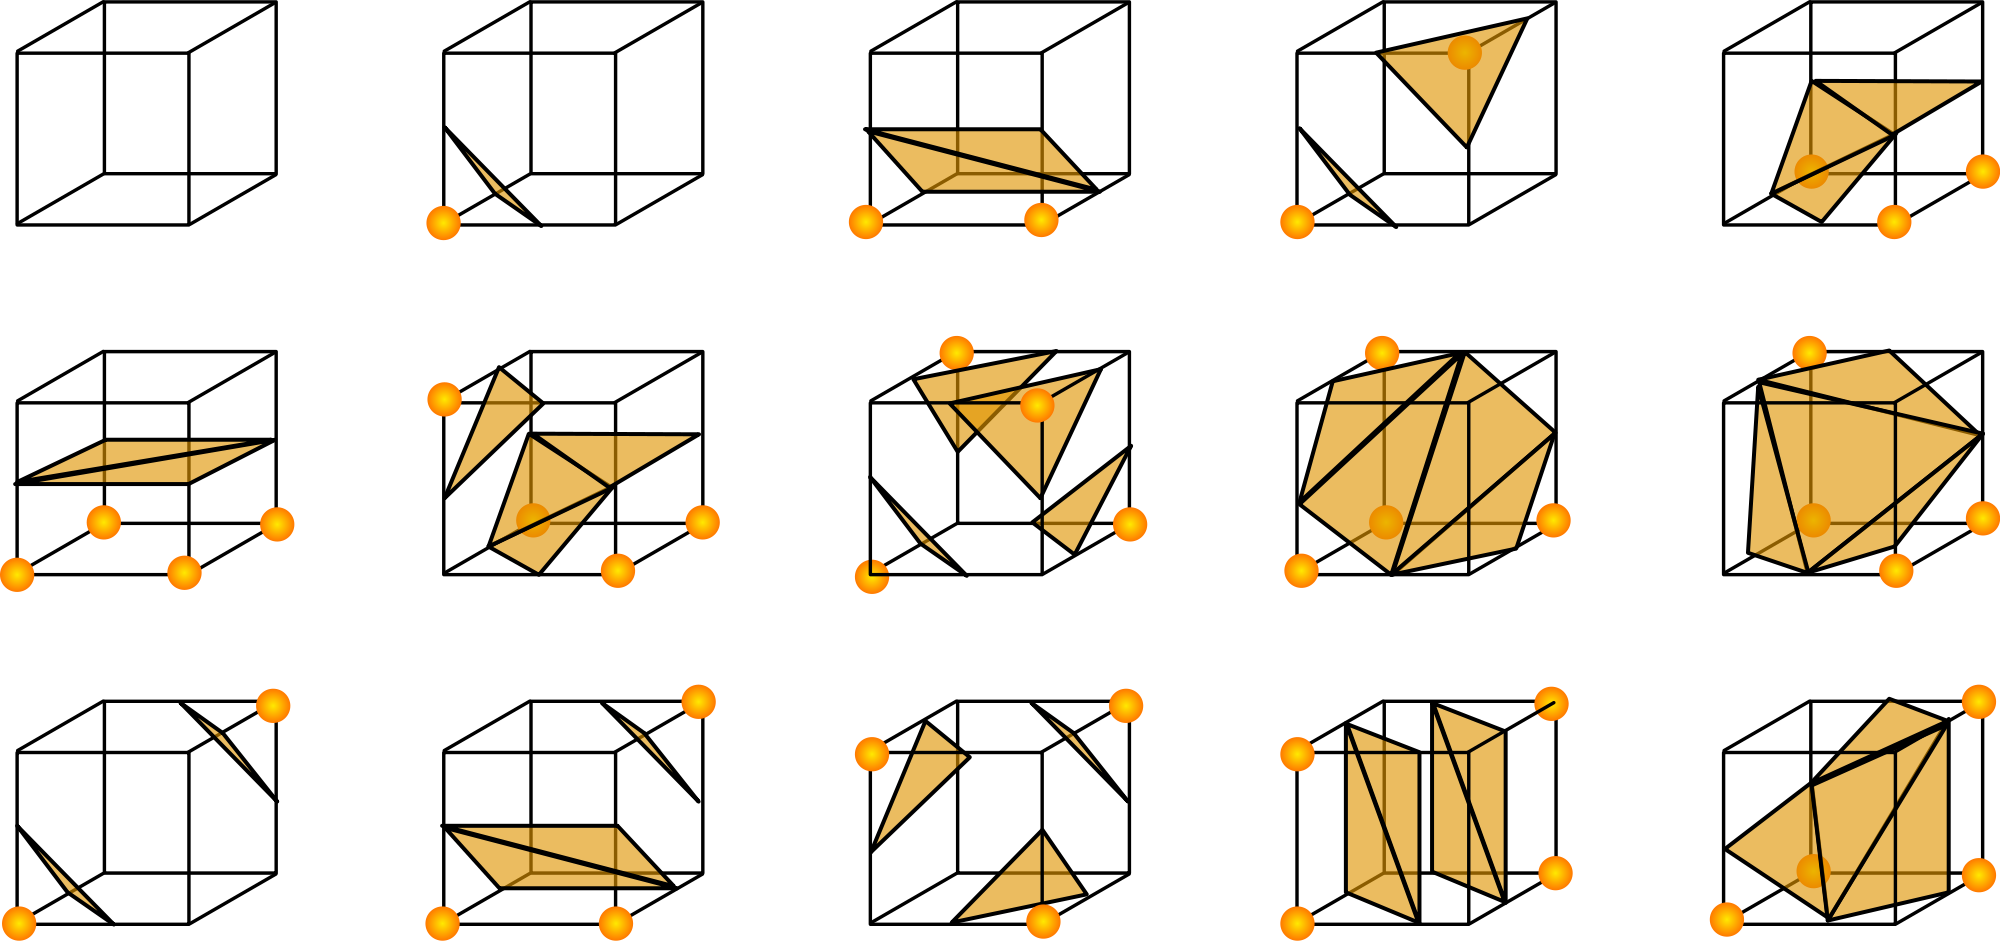
\includegraphics[width=.75\textwidth]{img/mcpolys}
	\caption{Le 15 configurazioni originali di Marching Cubes.}
	\label{fig:mcpolys}
\end{figure}

Marching Cubes lavora su un parallelepipedo alla volta per il quale ha a disposizione un array di $256$ ($ = 2^{\text{\# di vertici di un voxel}}$) possibili configurazioni, differenziate sulla base dei vertici interni ed esterni alla superficie da ricostruire. Ognuna di queste configurazioni prevede la definizione di uno o più triangoli, i cui vertici risiedono sugli spigoli del parallelepipedo stesso. La posizione di questi punti può essere scelta in base ad una funzione che ``pesa'' la vicinanza della superficie da rappresentare ai vertici del parallelepipedo ma, nell'implementazione realizzata, viene sempre usato il punto medio dello spigolo: questa scelta permette di risparmiare molta memoria sull'octree del \emph{miller} ed è ulteriormente motivata dal fatto che l'aumento della precisione nella visualizzazione dovrebbe essere ottenuto solo riducendo la dimensione del voxel usato nella simulazione.

\subsubsection{Sviluppi futuri.}
La figura \ref{fig:meshing_octree} mostra che garantire performance $O(1)$ nella cancellazione e nell'aggiornamento di dati costa molto in termini di spazio occupato, in quanto necessita di una lista doppiamente concatenata e, per ciascun voxel salvato, di una coppia di \emph{shared pointer}.
\begin{figure}[htp]
	\centering
	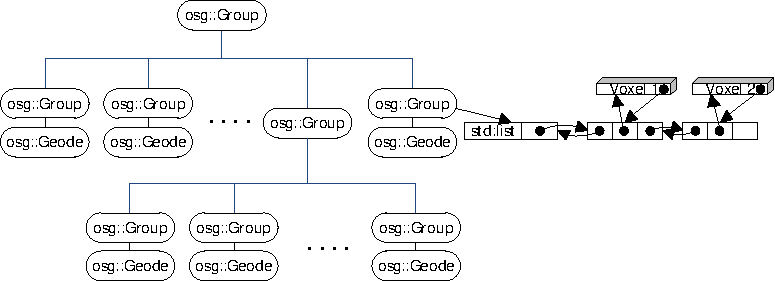
\includegraphics[width=.85\textwidth]{img/meshing_octree}
	\caption{Octree usato dal mesher per visualizzare l'oggetto lavorato.}
	\label{fig:meshing_octree}
\end{figure}
Un possibile sviluppo futuro consiste nel portare le operazioni di cancellazione e aggiornamento a complessità logaritmica, limitando la prima fase a marcare come ``modificate'' quelle liste di voxel interessate dai cambiamenti; sarà poi la seconda fase che si occuperà di riallineare il contenuto dell'albero con lo stato di fatto. Così facendo le liste possono essere sostituite da array e le coppie di \emph{shared pointer} con singoli \emph{weak pointer}\footnote{I concetti di \emph{shared} e \emph{weak pointer} sono mutuati dalla libreria boost e spiegati nella relativa documentazione, reperibile all'url \url{http://www.boost.org/doc/libs/1_52_0/libs/smart_ptr/smart_ptr.htm}} che puntano al voxel, risparmiando così memoria RAM.

Una strada che non è stata praticata consiste nell'uso di \cuda per le operazioni di meshing. Date le peculiarità del calcolo parallelo su scheda grafica\footnote{Un algoritmo che sfrutta in maniera ottimale il pipelining offerto dal calcolo su GPU riduce al minimo il numero di salti condizionati, e usa in modo intensivo i dati forniti in input: questi sono i motivi per cui è stata abbandonata l'idea di sfruttare \cuda anche nel \emph{milling}.}, la generazione delle mesh potrebbe trarre vantaggio dalla potenza di calcolo messa a disposizione da queste librerie, a patto di prestare attenzione a come i dati vengono scambiati tra la memoria di sistema e quella grafica: questi trasferimenti, infatti, possono diventare velocemente un collo di bottiglia per l'algoritmo.
